\setstretch{1.5}
\clearpage
\section{Χαρακτηριστικά εκδόσεων \en{OpenMP} 3.0 - 4.5}
Η έκδοση του \emph{\en{OpenMP}} που ακολούθησε της 2.5, ήταν η 3.0. Η νέα έκδοση περιείχε σημαντικές προσθήκες και
αλλαγές για τα δεδομένα του παράλληλου προγραμματισμού. Χαρακτηριστικά προηγούμενων εκδόσεων αναβαθμίστηκαν, ωστόσο τη
σημαντικότερη αλλαγή αποτέλεσε η εισαγωγή της έννοιας των εργασιών (\textbf{\en{Tasking}}). Η επόμενη έκδοση του
\emph{\en{OpenMP}} (4.0) κυκλοφόρησε τον Ιούλιο του 2013 και περιελάμβανε τα παρακάτω νέα χαρακτηριστικά:

\setlist[1]{itemsep=-5pt}
\begin{itemize}
    \item \emph{\en{Threads affinity}},
    \item Ετερογενής προγραμματισμός,
    \item Διαχείριση σφαλμάτων,
    \item Διανυσματικοποίηση μέσω \emph{\en{SIMD}},
    \item \emph{\en{User-Defined Recuctions (UDRs)}}
\end{itemize}

Τα τελευταία χρόνια η ανάγκη για εφαρμογές κατασκευασμένες με υψηλά επίπεδα παραλληλισμού είναι αυξημένη. Κύρια αιτία
αποτελεί η ευκολία πρόσβασης σε μεγάλο όγκο δεδομένων από το ευρύ κοινό, οι μικρές εξαρτήσεις ανάμεσά στα δεδομένα, αλλά
και η ανάγκη για εντατικούς υπολογισμούς στα δεδομένα αυτά. Λύση στο πρόβλημα αυξημένου φόρτου υπολογισμών αποτελεί η
χρήση ετερογενών συστημάτων προγραμματισμού. Ωστόσο, παρά τα οφέλη της υλοποίησης και χρήσης τέτοιων συστημάτων σε ότι
αφορά την απόδοση, ο προγραμματισμός εφαρμογών σε αυτά, δρα ανασταλτικά για την ευρεία χρήση τους. Το \emph{\en{OpenMP}}
δημιούργησε τα κατάλληλα εργαλεία για την εξάλειψη δυσκολιών υλοποίησης. Με τη δημοσίευση της έκδοσης 4.0, προσέφερε την
υποδομή για την υποστήριξη ετερογενών συστημάτων, καθώς η έκδοση περιλαμβάνει ένα σύνολο οδηγιών και φράσεων τα οποία
χρησιμοποιούνται για τον προσδιορισμό ρουτινών και δεδομένων, ικανών να μετακινηθούν σε μια συσκευή στόχου
(επιταχυντή) για να υπολογιστούν. Στόχος είναι η αύξηση των επιδόσεων υπολογισμού αλλά και η μείωση της κατανάλωσης
ισχύος. 

Εκτός από την υποστήριξη ετερογενών συστημάτων, το \emph{\en{OpenMP}} υποστηρίζει την επεξεργασία δεδομένων μέσω
διανυσματικοποίησης \emph{\en{SIMD}}. Η επεξεργασία \emph{\en{SIMD (Simple Instruction Multiple Data)}} εκμεταλλεύεται
τον παραλληλισμό σε επίπεδο δεδομένων, πράγμα που σημαίνει ότι οι πράξεις που γίνονται σε ένα σύνολο μιας συστοιχίας γίνονται ταυτόχρονα μέσω απλών εντολών.

Στις ενότητες του κεφαλαίου που ακολουθούν, εκτός από την αναλυτικότερη περιγραφή των παραπάνω βασικών χαρακτηριστικών,
γίνεται περιγραφή της έννοιας του \emph{\en{Thread Affinity}}, των \emph{\en{User-Defined Reductions}} και των
εργασιών\emph{\en{(Tasking)}}.

\clearpage
\subsection{Διανυσματικοποίηση μέσω \emph{\en{SIMD}}}
Κατά την διάρκεια εκτέλεσης ενός τυπικού προγράμματος από έναν μη παράλληλο υπολογιστή, οι εντολές που εκτελούνται είναι
απλές, εφαρμοζόμενες σε απλά, μοναδιαία δεδομένα. Το μοντέλο αυτό ονομάζεται (\emph{\en{SISD - Single Instruction Single
Data}}) και αποτελούσε για πολλά χρόνια το επικρατέστερο μοντέλο υλοποίησης και εκτέλεσης προγραμμάτων.
Αποτελεί ένα από τα τέσσερα μοντέλα της ταξινόμησης \emph{\en{Flynn}} που προτάθηκε το 1966\cite{flynn}. Τα άλλα τρία
μοντέλα είναι: 
\begin{itemize}
\item{\emph{\en{SIMD - Single Instruction Multiple Data}}}
\item{\emph{\en{MISD - Multiple Instruction Single Data}}}
\item{\emph{\en{MIMD - Multiple Instructions Multiple Data}}}
\end{itemize}


Στο μοντέλο \emph{\en{Single Instruction Multiple Data (SIMD)}}, εκτελούνται απλές λειτουργίες για την διαχείριση ενός
συνόλου δεδομένων τοποθετημένων στη σειρά. Το σύνολο αυτών των δεδομένων ονομάζεται πίνακας.

Στο παρακάτω σχήμα παρουσιάζεται η πρόσθεση των στοιχείων δυο πινάκων και η εκχώρηση των αποτελεσμάτων σε ένα τρίτο,
με τον συμβατικό τρόπο και με την χρήση \emph{\en{SIMD}} μεθόδου. Το πλεονέκτημα της δεύτερης μεθόδου είναι ότι οι
\emph{\en{SIMD}} οδηγίες εκτελούνται το ίδιο γρήγορα με τις αντίστοιχες βαθμωτές. Με άλλα λόγια η πράξη του σχήματος, θα
γίνει 4 φορές πιο γρήγορα στη δεύτερη περίπτωση.

\begin{figure}[h]
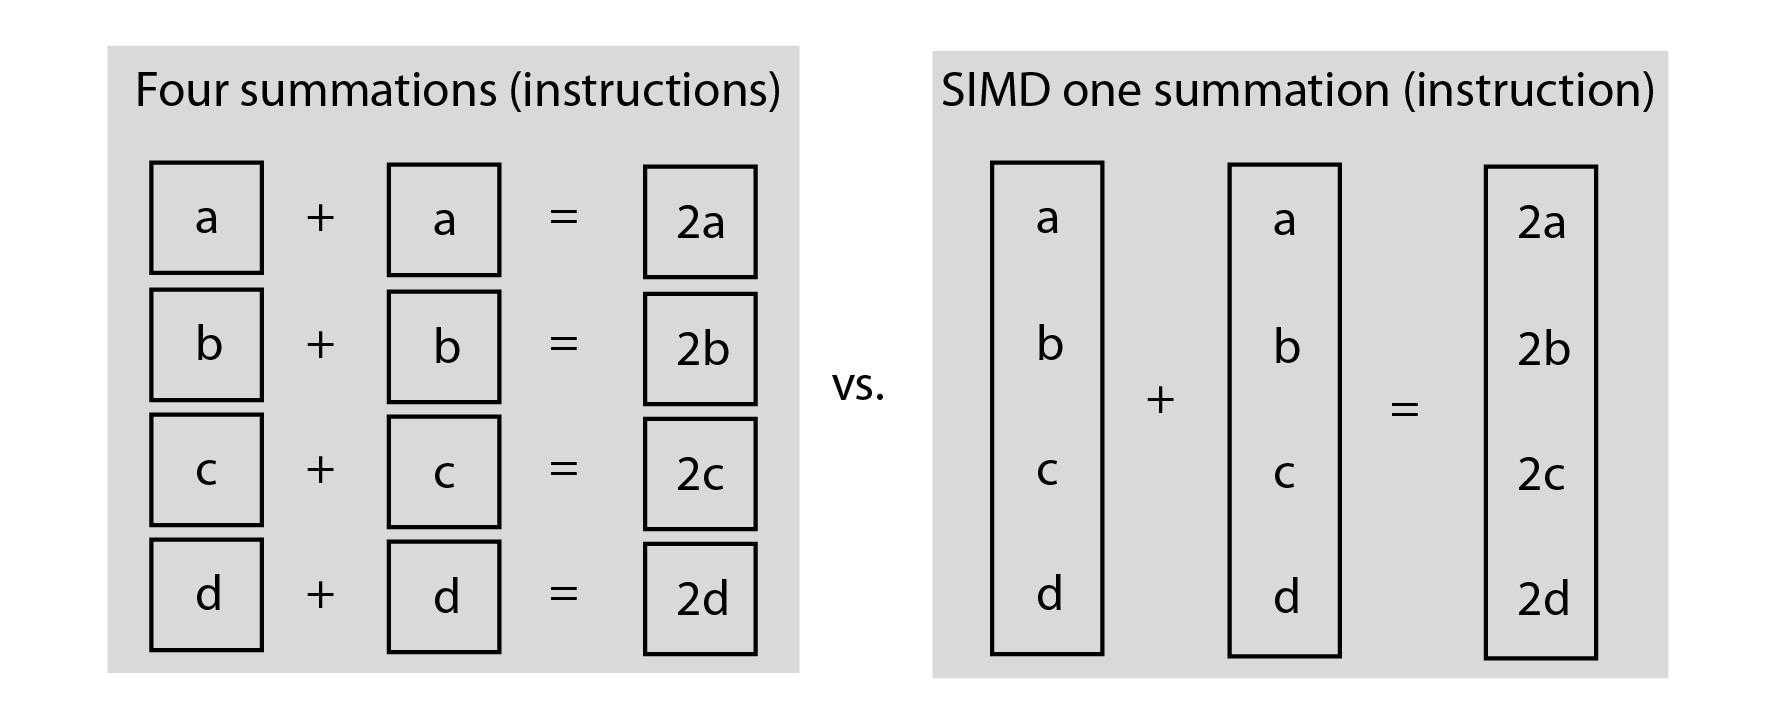
\includegraphics[width=0.8\textwidth]{scalar_vs_simd}
\centering
\captionsetup{justification=centering, singlelinecheck=false}
	\caption{ Πρόσθεση πινάκων βαθμωτά και με διανυσματικοποίηση}
\label{fig:scalar_vs_simd}
\end{figure}

 Στο κεφάλαιο αυτό, περιγράφονται τα χαρακτηριστικά και οι δυνατότητες που είναι διαθέσιμες στο \emph{\en{OpenMP}} και
 αφορούν λειτουργίες διανυσματικοποίησης μέσω \emph{\en{SIMD}}. 

\clearpage
\subsubsection{Η οδηγία \emph{\en{simd}}}
Αν ο μεταγλωττιστής δεν εφαρμόζει διανυσματικοποίηση ή δεν χρησιμοποιείται κάποια ειδική βιβλιοθήκη, τότε η επόμενη
καλύτερη μέθοδος διανυσματικοποίησης είναι με τη χρήση του \emph{\en{OpenMP}}. Η διεπαφή εφοδιάζει το χρήστη με ένα
σύνολο οδηγιών και φράσεων που σκοπό έχουν να ενημερώσουν το μεταγλωττιστή, να εκτελέσει παράλληλα ή με
διανυσματικοποίηση βρόγχους επανάληψης.

Βασικότερη οδηγία της διεπαφής αποτελεί η \textbf{\emph{\en{simd}}}. Εφαρμόζεται σε βρόγχους των οποίων η δομή είναι
ίδια με την δομή των κοινών βρόγχων της \emph{\en{C++}}. Η εισαγωγή της οδηγίας \emph{\en{simd}} δίνει εντολή στο
μεταγλωττιστή να δημιουργήσει έναν \emph{\en{simd}} βρόγχο.

Ιδιαίτερη προσοχή απαιτείται σε περιπτώσεις χρήσης  μεταβλητών όπως δείκτες μέσα στο βρόγχο. Η λανθασμένη χρήση τους
μπορεί να προκαλέσει απροσδιόριστη συμπεριφορά. Για παράδειγμα, στο παρακάτω τμήμα κώδικα, αν ο δείκτης \emph{\en{k}} ή
\emph{\en{m}} είναι ταυτόσημος με τον δείκτη t, τότε αναμένονται λάθος αποτελέσματα. 
\selectlanguage{english}

\begin{lstlisting}[language=C++, caption={\el{Εφαρμογή οδηγίας} simd} , frame=tb]{Name}
void accumulate(int *t, int *k, int *m, int n) {
	#pragma omp simd
	for (int i = 0; i < n; ++i) {
		t[i] = k[i] + m[i];
	}
}
\end{lstlisting}
\selectlanguage{greek}


Στο παράδειγμα, η μεταβλητή \emph{\en{i}} είναι ιδιωτική.
Σε ένα τσιπ υπάρχουν πολλοί πυρήνες που μπορούν να τρέξουν ταυτόχρονα. Μέσα σε έναν πυρήνα, υπάρχουν πολλά νήματα που τρέχουν ταυτόχρονα, και μέσα σε ένα νήμα υπάρχουν λωρίδες \en{SIMD}.
Η διαφορά με την ιδιωτική μεταβλητή ενός παράλληλου βρόγχου
είναι ότι η ιδιωτικότητα αναφέρεται στη λωρίδα \emph{\en{SIMD - (SIMD lane)}}. Οι τιμές των πινάκων \emph{\en{t, k, m}} είναι
κοινόχρηστες. Το καταλληλότερο μέγεθος πίνακα για την διανυσματικοποίηση, εξαρτάται από την αρχιτεκτονική του
μηχανήματος και επιλέγεται από αυτό. 
\subsubsection{Φράσεις οδηγίας \emph{\en{simd}}}
Ένα σύνολο φράσεων ακολουθούμενων της οδηγίας \emph{\en{simd}} υποστηρίζεται από το \emph{\en{OpenMP}}. Οι φράσεις
\emph{\en{private, lastprivate, reduction, collapse, ordered}}, έχουν την ίδια χρησιμότητα που προαναφέρθηκε στην
οδηγίες των προηγούμενων κεφαλαίων(πχ οδηγία διαμοιρασμού βρόγχου). Το σύνολο των φράσεων που υποστηρίζονται από την
οδηγία εμφανίζονται παρακάτω:
\selectlanguage{english}
\begin{lstlisting}[language=C++, caption={\el{Φράσεις οδηγίας} \emph{simd}} , frame=tlrb]{Name}
private (list)
lastprivate (list)
reduction (reduction-identifier : list)
collapse (n)
simdlen (length)
safelen (length)
linear (list[: linear-step J)
aligned (list{:alignment])
\end{lstlisting}
\selectlanguage{greek}

\paragraph{\underline{Φράση \en{simdlen}}}
\ \\
Η φράση \emph{\en{simdlen}} δέχεται ως όρισμα ένα θετικό ακέραιο αριθμό που καθορίζει τον προτιμώμενο αριθμό επαναλήψεων
ενός βρόγχου που θα εκτελούνται ταυτόχρονα. Επηρεάζει το μήκος του πίνακα που χρησιμοποιείται από τις παραγόμενες
\emph{\en{simd}} οδηγίες.

Η τιμή του ορίσματος είναι προτιμητέα αλλά όχι υποχρεωτική. Ο μεταγλωττιστής έχει την ελευθερία να αποκλίνει από αυτή
την επιλογή και να επιλέξει διαφορετικό μήκος. Ελλείψει αυτής της φράσης ορίζεται μια προεπιλεγμένη τιμή που καθορίζεται
από το μεταγλωττιστή. Σκοπός της φράσης \emph{\en{simdlen}} είναι να καθοδηγήσει τον μεταγλωττιστή. Χρησιμοποιείται από
τον χρήστη όταν έχει καλή εικόνα των χαρακτηριστικών του βρόγχου και γνωρίζει όταν κάποιο συγκεκριμένο μήκος μπορεί να
ωφελήσει στην απόδοση.
\clearpage
\paragraph{\underline{Φράση \en{safelen}}}
\mbox{}\\
Η φράση \emph{\en{safelen}} δέχεται ως όρισμα ένα θετικό ακέραιο αριθμό. Η τιμή αυτή καθορίζει το ανώτατο όριο του
μεγέθους πίνακα. Είναι το μήκος το οποίο είναι ασφαλές για τον βρόγχο. Το τελικό μέγεθος πίνακα επιλέγεται από τον
μεταγλωττιστή, αλλά δεν υπερβαίνει ποτέ την τιμή της φράσης \emph{\en{safelen}}.

Στο παρακάτω παράδειγμα απαιτείται η φράση \emph{\en{safelen}}. Πρόκειται για έναν βρόγχο που περιέχει εξάρτηση(\en{dependence}) στην
προσπέλαση των στοιχείων του πίνακα. Πιο συγκεκριμένα, το διάβασμα του \emph{\en{[i-10]}} στην επανάληψη
\emph{\en{i}} δεν μπορεί να υλοποιηθεί, αν δεν ολοκληρωθεί η εγγραφή στο \emph{\en{k[i]}} της προηγούμενης επανάληψης.
 
\selectlanguage{english}

\begin{spacing}{1.3}
\begin{lstlisting}[language=C++, caption={\el{Παράδειγμα κώδικα με} simd} , frame=tb]{Name}
void dep_loop(float *k, float c, int n) {
#pragma omp simd safelen(10)
	for (int i=10; i<n; i++) {
		k[i] = k[i-10] * c;
	}
}
\end{lstlisting}
\end{spacing}
\selectlanguage{greek}

\paragraph{\underline{Φράση \en{linear}}}
\mbox{}\\
Όταν χρησιμοποιείται σε περιβάλλον βρόχου \en{SIMD}, η φράση \en{linear} εκτελεί γραμμική αύξηση σε μια μεταβλητή
χρησιμοποιώντας \en{SIMD} οδηγίες. Η φράση \en{linear} παίρνει μια ακέραια μεταβλητή και προσθέτει το γραμμικό βήμα στη
μεταβλητή σε κάθε επανάληψη του βρόγχου. Η διαδικασία εξελίσσεται με τη δημιουργία δύο ιδιωτικών πινάκων εντός του
βρόχου \en{SIMD}. Ο πρώτος πίνακας περιέχει τη γραμμική ακολουθία που δημιουργήθηκε προσθέτοντας την τιμή βήματος στην
αρχική τιμή της μεταβλητής. Ο δέυτερος πίνακας περιέχει το γραμμικό βήμα που αυξάνει τον προηγούμενο πίνακα. Για
παράδειγμα, εάν η φράση έχει μια γραμμική μεταβλητή N = 1 με ένα γραμμικό βήμα 2 και χρησιμοποιείται έναν πίνακα
τεσσάρων θέσεων, τότε ο πρώτος ιδιωτικός πίνακας θα περιείχε 1, 3, 5, 7. Μετά από μια άλλη επανάληψη σε βρόχο \en{SIMD}, ο
πίνακας θα ήταν 9, 11, 13, 15. Αυτό γίνεται με την προσθήκη ενός διανύσματος που περιέχει 8, 8, 8, 8 μετά
από κάθε \en{SIMD lane}\cite{simd_linear}.


\paragraph{\underline{Φράση \en{aligned}}}
\ \\
Η ευθυγράμμιση των δεδομένων είναι σημαντική για την καλή απόδοση του προγράμματος. Αν ένα στοιχείο πίνακα δεν
είναι ευθυγραμμισμένο σε διεύθυνση μνήμης που είναι πολλαπλάσιο του μεγέθους του στοιχείου σε \emph{\en{byte}},
προκύπτει ένα επιπλέον κόστος καθυστέρησης για την τροποποίηση του στοιχείου αυτού.

Για παράδειγμα, σε ορισμένες αρχιτεκτονικές ενδέχεται να μην είναι δυνατή η φόρτωση και εγγραφή από μια διεύθυνση μνήμης
που δεν είναι ευθυγραμμισμένη με το μέγεθος του δεδομένου που χρησιμοποιείται. Έτσι, οι λειτουργίες γίνονται κανονικά,
αλλά με μεγαλύτερο κόστος. Σε περίπτωση διανυσματικοποίησης μέσω της οδηγίας \emph{\en{simd}}, η επιλογή ευθυγράμμισης
δεδομένων μπορεί να βελτιώσει την εκτέλεση.

Η φράση ευθυγράμμισης υποστηρίζεται τόσο από την οδηγία \emph{\en{simd}} όσο και από την οδηγία \emph{\en{declare
simd}}. Η φράση δέχεται ως όρισμα μια λίστα μεταβλητών. Η τιμή της ευθυγράμμισης πρέπει να είναι ένας σταθερός ακέραιος
αριθμός. Σε περίπτωση έλλειψης της φράσης, μια προεπιλεγμένη τιμή καθορίζεται από την υλοποίηση.
\ \\
\subsubsection{Η σύνθετη οδηγία βρόγχου \emph{\en{SIMD}}}
Η σύνθετη οδηγία βρόγχου \emph{\en{SIMD}}, συνδυάζει παραλληλισμό νημάτων και διανυσματικοποίηση μέσω \emph{\en{SIMD}}.

\begin{spacing}{1.1}
\selectlanguage{english}
\begin{lstlisting}[language=C++, caption={\el{Γραμματική οδηγίας \en{omp for simd}}} , frame=tlrb]{Name}
#pragma omp for simd [clause[[,] clause] ...] new-line
	for-loops
\end{lstlisting}
\selectlanguage{greek}
\end{spacing}
\ \\
Οι επαναλήψεις ενός βρόγχου διαιρούνται σε τμήματα και διανέμονται σε μια ομάδα νημάτων. Στη συνέχεια, τα τμήματα αυτά
εκτελούνται βάση της οδηγίας επαναληπτικού \emph{\en{simd}} βρόγχου. Οι φράσεις που μπορούν να χρησιμοποιηθούν στην
οδηγία διαμοιρασμού βρόγχου ή στην οδηγία \emph{\en{simd}} μπορούν να χρησιμοποιηθούν και σε αυτές τις σύνθετες οδηγίες.

Στη σύνθετη οδηγία, τμήματα επαναλήψεων του βρόγχου διανέμονται στην ομάδα νημάτων με τη μέθοδο που ορίζουν οι φράσεις
διαμοιρασμού που χρησιμοποιούνται στην οδηγία διαμοιρασμού επαναλήψεων. Στη συνέχεια, τα τμήματα επαναλήψεων βρόγχου
μετατρέπονται σε οδηγίες \emph{\en{simd}} με μέθοδο που ορίζεται από τις φράσεις για την οδηγία \emph{\en{simd}}. Τα
παραπάνω φαίνονται σχηματικά στην επόμενη εικόνα:
\ \\
\begin{figure}[h]
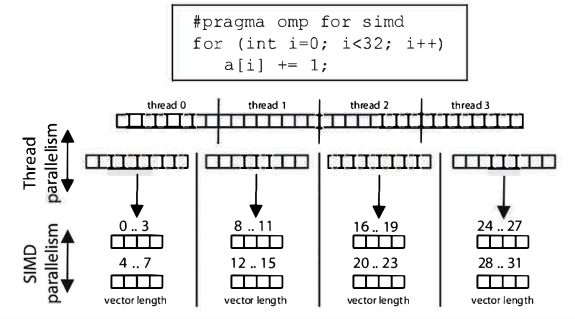
\includegraphics[width=0.9\textwidth]{for_simd}
\centering
\captionsetup{justification=centering, singlelinecheck=false}
	\caption{ Βήματα εργασιών οδηγίας \emph{\en{for simd}}}
\label{fig:for_simd}
\end{figure}

Κάθε νήμα ενός επαναληπτικού βρόγχου έχει ένα συγκεκριμένο ποσοστό εργασίας που πρέπει να εκτελέσει. Αν ο αριθμός των
νημάτων αυξηθεί, το ποσοστό της εργασίας ανά νήμα θα μειωθεί. Προσθέτοντας παραλληλισμό \emph{\en{simd}}, δεν είναι
απαραίτητη η βελτίωση της απόδοσης, ειδικά στις περιπτώσεις που ο επαναληπτικός \emph{\en{simd}} βρόγχος που ανήκει σε
ένα νήμα μειώσει το μήκος του.
\clearpage{}

\subsubsection{Συναρτήσεις \emph{\en{SIMD}}}
Οι κλήσεις συναρτήσεων εντός της περιοχής βρόγχου \emph{\en{SIMD}} εμποδίζουν τη δημιουργία αποτελεσματικών
\emph{\en{SIMD}} δομών. Στη χειρότερη περίπτωση η κλήση της συνάρτησης θα γίνει χρησιμοποιώντας βαθμωτά δεδομένα, κάτι
που πιθανότατα θα επηρεάσει αρνητικά την αποτελεσματικότητα.

Για την πλήρη εκμετάλλευση του παραλληλισμού με διανυσματικοποίηση, για κάθε συνάρτηση που καλείται μέσα από ένα βρόγχο
\emph{\en{SIMD}}, πρέπει να ορίζεται μια ισοδύναμη έκδοσή της για εκτέλεση μέσα σε βρόγχους \emph{\en{SIMD}}. Έτσι, ο
μεταγλωττιστής θα δημιουργήσει αυτή την ειδική έκδοση της συνάρτησης με \emph{\en{SIMD}} παραμέτρους και οδηγίες.

Η οδηγία \emph{\en{ declare simd}} χρησιμοποιείται για να δημιουργήσει ο μεταγλωττιστής μια ή περισσότερες εκδόσεις μιας
συνάρτησης. Οι εκδόσεις αυτές χρησιμοποιούνται αποκλειστικά από βρόγχους \emph{\en{SIMD}}.


\paragraph{H οδηγία \emph{\en{declare simd}}}
\ \\
Η οδηγία \emph{\en{declare simd}} χρησιμοποιείται για να ενημερωθεί ο μεταγλωττιστής ότι μια συνάρτηση μπορεί να
χρησιμοποιηθεί από μια περιοχή παραλληλισμού \emph{\en{simd}}.

\begin{spacing}{1.1}
\selectlanguage{english}
\begin{lstlisting}[language=C++, caption={\el{Γραμματική οδηγίας} \emph{declare simd}} , frame=tlrb]{Name}
#pragma omp declare simd [clause [[,] clause] ...] new-line
	function declaration definitions
\end{lstlisting}
\selectlanguage{greek}

\selectlanguage{english}
\begin{lstlisting}[language=C++, caption={\el{Φράσεις οδηγίας} \emph{declare simd}} , frame=tlrb]{Name}
simdlen (length)
linear (list[: linear-step J)
aligned (list[:alignmentj)
uniform ( argument-list)
inbranch
notinbranch
\end{lstlisting}
\end{spacing}
\selectlanguage{greek}

Ο μεταγλωττιστής μπορεί να δημιουργήσει πολλές \emph{\en{simd}} εκδόσεις  μιας συνάρτησης και να επιλέξει την κατάλληλη
για να κληθεί στο \emph{\en{simd}} τμήμα. Από τη μεριά του, ο χρήστης μπορεί να
προσαρμόσει την λειτουργία μιας συνάρτησης με τη χρήση εξειδικευμένων φράσεων.

Υπάρχουν ωστόσο δύο περιορισμοί. Αν μια μεταβλητή αλλάζει ως αποτέλεσμα μιας τροποποίησης μιας φαινομενικά άσχετης
μεταβλητής η συμπεριφορά είναι απροσδιόριστη. Επιπλέον, μια συνάρτηση που εμφανίζεται κάτω από οδηγία \emph{\en{declare
simd}} δεν επιτρέπει τα \emph{\en{exceptions}}.

\subsubsection{Χαρακτηριστικά παραμέτρων \emph{\en{SIMD}} συναρτήσεων}
Οι φράσεις \textbf{\emph{\en{uniform, linear, simdlen, aligned}}} χρησιμοποιούνται για τον καθορισμό χαρακτηριστικών στις
παραμέτρους μιας \emph{\en{simd}} συνάρτησης. Εκτός από την \emph{\en{simdlen}}, οι μεταβλητές που εισάγονται
στις υπόλοιπες φράσεις πρέπει να είναι παράμετροι της συνάρτησης για την οποία εφαρμόζεται η οδηγία.

Όταν μια παράμετρος εμπεριέχεται στη φράση \emph{\en{uniform}}, η τιμή της παραμέτρου είναι σταθερή για όλες τις
ταυτόχρονες κλήσεις κατά την εκτέλεση της οδηγίας \emph{\en{simd}} βρόχου. Η φράση \textbf{\en{uniform(arg1, arg2)}}
δίνει την οδηγία στο μεταγλωττιστή να δημιουργήσει μια \emph{\en{simd}} συνάρτηση που προϋποθέτει ότι αυτές οι δύο
μεταβλητές είναι ανεξάρτητες από τον βρόγχο. 

\selectlanguage{english}
\begin{spacing}{0.9}
\begin{lstlisting}[language=C++, caption={\el{Χρήση φράσεων \en{uniform - simdlen}}} , frame=tb]{Name}
#pragma omp declare simd simdlen(16) uniform(a, b, offset)
float do_work(float *a, float *b, int i, int offset)
{
	return a[i] ? a[i] + b[i] : b[i + offdset];
}
void fun(float *a, float *b, int offset, int len)
{
#pragma omp simd  aligned(a:64, b:64)
	for(int i = 0; i < len; i++)
 	{
 		a[i] = do_work(a, b, i, off);
 	}
}

\end{lstlisting}
\end{spacing}
\selectlanguage{greek}


Η φράση \emph{\en{linear}} ορίζει ότι ένα όρισμα που μεταβιβάζεται σε μια συνάρτηση έχει γραμμική σχέση μεταξύ των
παράλληλων επικλήσεων μιας συνάρτησης. Κάθε \emph{\en{simd lane}} παρατηρεί την τιμή του ορίσματος στην πρώτη λωρίδα και
προσθέτει την μετατόπιση της \emph{\en{simd}} λωρίδας από την πρώτη, επί το γραμμικό βήμα.
$$val_{curr} = val_1 + offset * step $$


\selectlanguage{english}
\begin{spacing}{0.8}
\begin{lstlisting}[language=C++, caption={\el{Χρήση φράσεων \en{uniform - simdlen}}} , frame=tb]{Name}
#pragma omp declare simd simdlen(16) uniform(a, b, offset)
float do_work(float *a, float *b, int i, int offset)
{
	return a[i] ? a[i] + b[i] : b[i + offdset];
}
void fun(float *a, float *b, int offset, int len)
{
#pragma omp simd  aligned(a:64, b:64)
	for(int i = 0; i < len; i++)
 	{
 		a[i] = do_work(a, b, i, off);
 	}
}

\end{lstlisting}
\end{spacing}
\selectlanguage{greek}


Η φράση \en{aligned} δηλώνει ότι το αντικείμενο στο οποίο κάθε σημείο της λίστας δείχνει, είναι ευθυγραμμισμένο με τον αριθμό των \en{byte} που δηλώνονται στην φράση. Ο αριθμός της πρέπει να είναι μια θετική ακέραια έκφραση.

Η φράση \emph{\en{inbranch}} χρησιμοποιείται όταν μια συνάρτηση καλείται πάντα μέσα σε ένα \emph{\en{simd}} βρόγχο και
περιέχει \emph{\en{if condition}}. Ο μεταγλωττιστής πρέπει να αναδιαρθρώσει τον κώδικα για να χειριστεί την πιθανότητα
ότι μια λωρίδα \emph{\en{simd}} μπορεί να μην εκτελέσει τον κώδικα μιας συνάρτησης.

Αντίθετα, η φράση \emph{\en{notinbranch}} χρησιμοποιείται όταν η συνάρτηση δεν εκτελείται ποτέ μέσα από ένα \emph{\en{if
condition}} σε ένα \emph{\en{simd}} βρόγχο. Επιτρέπει τον μεταγλωττιστή κάνει μεγαλύτερες βελτιστοποιήσεις στην απόδοση
του κώδικα μιας συνάρτησης που χρησιμοποιεί \emph{\en{simd}} οδηγίες.
\selectlanguage{english}
\begin{spacing}{0.8}
\begin{lstlisting}[language=C++, caption={\el{Χρήση φράσεων} inbranch - notinbranch} , frame=tb]{Name}
#pragma omp declare simd inbranch
float pow(float x) {
	return (x * x);
}

#pragma omp declare simd notinbranch
extern float div(float);

void simd_loop(float *a, float *b, int n)
{
	#pragma omp simd
	for (int i=0; i<n; i++) {
		if (a[i] < 0.0 )
			b[i] = pow(a[i]);
		b[i] = div(b[i]);
	}
}
\end{lstlisting}
\end{spacing}
\selectlanguage{greek}
